\documentclass{article}
\usepackage[T1]{fontenc}
\usepackage{setspace}
\usepackage[table]{xcolor}
\usepackage[margin=1in]{geometry}
\usepackage{tabularx}
\usepackage{enumitem}
\usepackage{hyperref,verbatim}
\setcounter{tocdepth}{3}
\setcounter{secnumdepth}{0}
\usepackage{array}
\usepackage{babel}
\usepackage{graphicx}
\usepackage{subfigure, wrapfig}
\usepackage{amssymb, amsmath}
\usepackage{tikz}
\usepackage{epsdice}
\usepackage[resetlabels,labeled]{multibib}
\usepackage{moeptikz}
\usepackage{pgfplots}
\onehalfspacing

\setlist{nolistsep}

\definecolor{blue}{HTML}{008ED7}
\definecolor{lightBlue}{HTML}{e5f7ff}
\newcommand{\n}{\cellcolor{green!10} not capable}
\newcommand{\y}{\cellcolor{purple!10} capable}

\renewcommand{\familydefault}{\sfdefault}
\renewcommand{\arraystretch}{1.5}

\title{Mixnet Research Review}
\author{E. J. Infeld and D. Stainton}


\newcites{M}{Mixnet design research}
\newcites{E}{Mixnet evaluation}
\newcites{A}{Selected sources on attacks}

\begin{document}

\maketitle
\begin{abstract}
\noindent We provide a selected overview of decades of research on Mixnets, with special focus on the modern solutions implemented in multiple actively developed projects, such as Katzenpost and Nym. The purpose of this work is to provide a resource on the general knowledge in this robust field. \smallskip

\noindent This work is supported by a grant from the Wau Holland Foundation.

\end{abstract}

\tableofcontents
\vfill

% XXX: First, I would _introduce_ mixnets before justifying why
\section{Why Mixnets? The need for systems that can protect from powerful adversaries.}

The strife for privacy in the modern world is inseparable from our need for freedom and sovereignty. It is no longer controversial to say that we face very powerful adversaries in this strife. These could be state, corporate or criminal actors, vying for our information to use as means of making profit, manipulating us and others, gaining leverage, strengthening their authority, or as means of persecution. In many contexts, we have little hope for non-technical solutions due to lack of sufficiently powerful pressure in favor of privacy.

In our quest for technical solutions, we need equally powerful tools. In the case of communication tools, the Internet's bread and butter, we would like to allow users to interact and exchange information with reasonable expectation of both the content and metadata of their communication, and personal information such as a user's social graph, being protected from such adversaries. %Simply encrypting the connection is no longer enough, as confirmed by extensive resources on critical information leaked by metadata, such [insert sources] as or even reconstructing sections of conversations in VoIP calls from packet traffic analysis. \citeA{phonemes} \citeA{phonemesdl}



If we hope for our work to be relevant in the modern world, we can no longer settle for weak threat models. Therefore, consider an adversary capable of the following:
\begin{itemize}
\item The adversary can see the traffic of the entire global internet, and in particular between devices in the network, and is capable of intricate statistical analysis of gathered data.
\item The adversary can disable parts of the network.
\item The adversary can plant or take over some devices in the network to inject malicious code and manipulate the functioning of the network or to gain access to the information available to them. The takeover could happen by technical means or by exercising force outside of the network.
\item The adversary has very large, but not infinite, computational resources, and is capable of cryptanalysis on par with frontier research.
\item The adversary has access to a quantum computer, or will have access to a quantum computer in the near future.
\item The adversary can supplement collected data with rich context of already gathered data on all users from other sources.
\end{itemize}

\noindent  We aim to rise up to the challenge with modern Mixnets.
\vfill

\pagebreak
\section{Mixnet basics}

A mix network is a collection of network devices, referred to as \textit{mix nodes}, that attempt to relay multiple messages from a set of senders to a set of receivers (these are typically the same set) in such a way that a third party observing the network is unaware of which sender is sending a message to which receiver. We will refer to these senders and receivers as either \textit{users} or \textit{clients} of the network. 

A \textit{batch mix} could for example have regularly scheduled rounds in which messages are collected and routed through several devices (\textit{hops}) in the network where each hop shuffles the messages. Therefore, it can be said that in a batch mix, the primary source of \textit{mix entropy} comes from the message shuffling, and indeed the entropy or the measure of the uncertainty a passive network observer would have in trying to link input messages with output messages, is a function of the batch size. On the other hand, \textit{continuous time mixing} strategies differ from batch mixnets because each message is delayed independently from the other messages which allows for a more favorable latency tradeoff as is the case with the Loopix design \citeM{loopix}. In such a strategy, the sampled delay must be probabilistic in nature, since a deterministic delay could be reconstructed by an adversary and used to correlate messages.\footnote{Randomness is in the eye of the beholder. It's enough if the delay is sampled in a way that appears random to the adversary.}

%The server stored a list of the users' pseudonyms and real addresses, much like post boxes. Should that server be compromised, both the destinations and the content of messages would be revealed. An early practical example of a simple mix was the Penet remailer, which operated from 1993 until being compromised by a compulsion attack\footnote{see attacks table on page \pageref{tab:attacks}} in 1996.\citeA{penet} 
%\subsection{Every protocol decision comes with consequences}

We would like to impress on the reader, that when designing networking protocols with strong adversaries in mind, every decision comes with trade-offs and consequences. Let us focus for now on a simple batch mix with a single mix node, that is relaying messages with the hopes of hiding from a network observer which of the incoming messages corresponds to which of the outgoing ones. Suppose we consider a setup in which Alice only has the mix node's public key, and encrypts her message to Bob with that, and the mix node decrypts it and then encrypts it again with Bob's public key. A straightforward improvement on that comes with nested encryption - if Alice wishes to send a message to Bob, she can encrypt the message with Bob's public key, add a note for the server where to send it, and then encrypt the encrypted message together with that note with the server's public key. The server can then pass the message onto Bob without knowing its content. The difference between the two simple setups is illustrated below - as Alice sends a message to Bob, and Charlie sends a message to Diane, and the mix server releases them both at once. A casual observer might not know whether that's what's happened, or if Alice sent a message to Diane, and Charlie to Bob.


\begin{figure}[!ht]
\centering\hfill
\begin{tikzpicture}[scale=0.75]\hfill
\draw[blue!50!black, ->, dashed] (-3.7,0)--(-0.6,0);
\draw[blue!50!black, <-, dashed] (3.5,0)--(0.6,0);
\node[client,minimum size=0.7cm, fill=purple] at (4,0.3) {};
\draw (-4,-0.3) node {Alice};
\draw (4,-0.3) node {Bob};
\node[client,minimum size=0.7cm] at (-4,0.3) {};
\node[messageclosed, minimum size = 0.5cm, fill=blue!30!white] at (-2,0) {};
\node[messageclosed, minimum size = 0.5cm, fill=purple!50!white] at (2,0) {};
\node[messageopen, minimum size=0.5cm, fill=blue!30!white] at (0,1) {};
\node[server, fill=blue!50!white] at (0,0) {};
\node[client,minimum size=0.7cm] at (-3,2) {};
\draw (-3,1.4) node {Charlie};
\node[client,minimum size=0.7cm] at (2.5,-1.4) {};
\draw (2.5,-2) node {Diane};
\draw[blue!50!black, ->, dashed] (-2.7,1.7)--(-0.6,0.2);
\draw[blue!50!black, <-, dashed] (1.9,-1.1)--(0.6,-0.2);
\node[messageclosed, minimum size=0.5cm, fill=green!50!white] at (1.25,-0.65) {};
\node[messageclosed, minimum size=0.5cm, fill=blue!30!white] at (-1.65,0.95) {};
\node[messageopen, minimum size=0.5cm, fill=blue!30!white] at (0,-1.05) {};
\end{tikzpicture}\hfill
\begin{tikzpicture}[scale=0.75]
\draw[blue!50!black, ->, dashed] (-3.7,0)--(-0.6,0);
\draw[blue!50!black, <-, dashed] (3.5,0)--(0.6,0);
\node[client,minimum size=0.7cm, fill=purple] at (4,0.3) {};
\draw (-4,-0.3) node {Alice};
\draw (4,-0.3) node {Bob};
\node[client,minimum size=0.75cm] at (-4,0.3) {};
\node[messageclosed, minimum size = 0.5cm, fill=purple!80!white] at (-2,0) {};
\node[messageclosed, minimum size = 0.8cm, fill=blue!50!white, opacity=0.3] at (-2,0.1) {};
\node[messageclosed, minimum size = 0.5cm, fill=purple!50!white] at (2,0) {};
\node[server, fill=blue!50!white] at (0,0) {};
\node[messageclosed, minimum size = 0.5cm, fill=purple!80!white] at (0,0.9) {};
\node[messageopen, minimum size = 0.8cm, fill=blue!50!white, opacity=0.3] at (0,1.1) {};
\node[client,minimum size=0.7cm] at (-3,2) {};
\draw (-3,1.4) node {Charlie};
\node[client,minimum size=0.7cm, fill=green] at (2.5,-1.4) {};
\draw (2.5,-2) node {Diane};
\draw[blue!50!black, ->, dashed] (-2.7,1.7)--(-0.6,0.2);
\draw[blue!50!black, <-, dashed] (1.9,-1.1)--(0.6,-0.2);
\node[messageclosed, minimum size=0.5cm, fill=green!50!white] at (1.25,-0.65) {};
\node[messageclosed, minimum size=0.5cm, fill=green!50!white] at (-1.65,0.95) {};
\node[messageclosed, minimum size = 0.8cm, fill=blue!50!white, opacity=0.3] at (-1.65,1.05) {};
\node[messageclosed, minimum size=0.5cm, fill=green!50!white] at (0,-1.05) {};
\node[messageopen, minimum size = 0.8cm, fill=blue!50!white, opacity=0.3] at (0,-0.95) {};
\end{tikzpicture}\hfill\hfill
\caption{%The server on the left decrypts all incoming messages, and encrypts them again for each receiver. The system on the right employs nested encryption. 
Blue envelopes are encrypted with the server's public key, red with Bob's and Green with Diane's.}
\label{Fig: Onion routing}
\end{figure}
\noindent This has the advantage of the server not learning the content of the messages, but it also has certain trade-offs. For example, each sender has to retrieve the final receiver's public key, possibly from the server. Also, a network observer could take a message going to Bob and try to recreate what it would have looked like coming into the server by using the server's public key, and then match it to a message sent by Alice. Alice can prevent this by adding a little randomness before encrypting the outer layer of the message, which the server will then strip. Similarly, for every improvement or addition we make to the system we will keep careful track of its consequences.


\subsection{Compromising on latency and compromising on bandwidth}
Let's now compare two simple \textit{mixing strategies} that one may encounter with mix nodes. A mixing strategy is the method which a mix node employs to attempt to hide from an adversary which of its users are communicating with each other. 

One, a mix node might collect many messages from multiple users, and then release them all at once, a batch mix. The hope is that an adversary will not be able to match a message being sent from a receiver to a message coming in from a sender. The batch mix scheduling and batch mix size (messages per batch) are tuned so that the desired latency/bandwidth 
tradefoff is achieved where the main cost is bandwidth since batch mixes always send an entire batch of messages. Since the adversary sees messages being sent, but doesn't know which outgoing messages correspond to which incoming ones, this strategy achieves sender-receiver \textit{unlinkability.} 

Two, a mix node might send decoy traffic between itself and the users with the overall traffic pattern independent of the amount of messages the users are sending, and the messages forming an indistinguishable subset of the traffic. In this method the main trade-off is the amount of bandwidth it uses. The adversary does not observe when a message is being sent, and therefore we say this strategy achieves \textit{unobservability.} We sometimes see protocols that have asymetric properties, where, for example, messages being sent are unobservable but messages being received are not, and vice versa. We then talk about \textit{sender unobservability} or \textit{receiver unobservability}, respectively.

\begin{figure}[!ht]
\centering
\hfill\begin{tikzpicture}[scale=1.5]
\foreach \x in {-1,0,1}{
\draw[opacity=1, dashed, blue!50!black, ->] (-2,\x) -- (-0.6,0.1*\x);
\draw[opacity=1, dashed, blue!50!black, <-] (1.5,\x) -- (0.5,0.1*\x);
\node[client,minimum size=0.7cm] at (-2,\x) {};
\node[client,minimum size=0.7cm] at (2,\x) {};
\node[messageclosed, minimum size=0.4cm, fill=cyan!30!white, draw=black!70] at (1,0.55*\x) {};}
\node[messageclosed, minimum size=0.4cm, fill=cyan!30!white, draw=black!70] at (-1,0) {};
\node[messageclosed, minimum size=0.4cm, fill=cyan!30!white, draw=black!70] at (-1.3,0.6) {};
\node[messageclosed, minimum size=0.4cm, fill=cyan!30!white, draw=black!70] at (-1.5,-0.75) {};
\node[server] at (0,0) {};
\end{tikzpicture}\hfill
\begin{tikzpicture}[scale=1.5]
\foreach \x in {-1,0,1}{
\filldraw[opacity=0.25, ultra thick, blue!30!black, ->] (-2,\x-0.2) -- (-0.6,0.1*\x-0.1) -- (-0.55,0.1*\x+0.1) -- (-2,\x+0.2);
\filldraw[opacity=0.25, ultra thick, blue!30!black, ->] (2,\x-0.2) -- (0.6,0.1*\x-0.1) -- (0.55,0.1*\x+0.1) -- (2,\x+0.2);
\node[client,minimum size=0.7cm] at (-2,\x) {};
\node[client,minimum size=0.7cm] at (2,\x) {};}
\node[messageclosed, minimum size=0.4cm, fill=cyan!30!white, draw=black!70] at (-1,0) {};
\node[messageclosed, minimum size=0.4cm, fill=cyan!30!white, draw=black!70] at (-1.35,0.6) {};
\node[messageclosed, minimum size=0.4cm, fill=cyan!30!white, draw=black!70] at (-1.5,-0.65) {};
\node[server] at (0,0) {};
\node[messageclosed, minimum size=0.4cm, fill=cyan!30!white, draw=black!70] at (1.55,0) {};
\node[messageclosed, minimum size=0.4cm, fill=cyan!30!white, draw=black!70] at (1.3,0.55) {};
\node[messageclosed, minimum size=0.4cm, fill=cyan!30!white, draw=black!70] at (1.1,-0.45) {};
\end{tikzpicture}\hfill\hfill
\caption{The system on the left compromises on latency. The system on the right compromises on bandwidth.}
\end{figure}

\noindent For a more sophisticated system, we would want to employ multiple independent mix nodes, and send a message through a sequence of them to prevent any one actor from correlating senders and receivers. This is where we go from a single mix node to a system deserving of the name \textit{mix network}. We would want to protect the messages with layers of encryption for each node, in much the same way it is done in Tor. However, Tor attempts to simulate the standard internet browsing experience, and therefore minimize latency and optimize bandwidth. It cannot afford to have its relays delay connections to properly mix them. It also cannot effectively employ decoy traffic or padding, since it wants its users to be able to take full advantage of their bandwidth at any given time, and padding to that level would be prohibitively expensive. This makes it vulnerable to adversaries capable of watching the network and correlating users' behavior. This is a \textit{statistical disclosure attack}, and we will elaborate on it in the next section. This vulnerability in Tor cannot be fixed if it is to keep its desired functionality.

 By contrast, a Mixnet does make these compromises in order to thwart powerful adversaries. Early designs attempted to ensure anonymity by compromising on latency rather than badwidth, while most modern Mixnet designs usually attempt find a sweet spot with the use of both. This means that some amount of traffic is being sent by a user at all times. The amount of traffic it allows for is also an upper limit to the user's bandwidth, since setting it too high would quickly add up to a significant drain on their resources. 

\pagebreak
 This recalls the Anonymity Trilemma - a rule that to maintain anonymity guarantees, you have to compromise either on the bandwidth overhead or on latency. It was systematized in \citeE{trilemma}. Some modern systems allow for tuning of both the latency and the bandwith overhead, and are therefore somewhat versatile. This includes Loopix \citeM{loopix}, where one could compensate for shortening the latency with increasing the bandwidth overhead and vice versa. In theory. In practice, user experience concerns are likely to constrain these choices.

Because of these compromises, some communication activities lend themselves to Mixnets more readily than others. Non-synchronous messaging, as with email, is a natural use case for this kind of an anonymity system. On the other hand, browsing the internet comfortably, as with Tor, appears to be impossible.



\section{Mixnet evolution}

%\subsection{Padding}

%Most modern Mixnet designs aim to thwart these powerful adversaries by introducing padding in order to mitigate traffic analysis. This allows them to limit the latency. The goal is to generate the padding in a way such that the traffic pattern of each node is independent of whether the traffic crossing through it consists of legitimate user connections or not, otherwise even the most naive statistical methods would render it useless.

%What this typically means in practice, is that the user, or sometimes a node, sends packets according to a set pattern, with any legitimate packets sent out first, and dummy packets being generated to fill up the rest of the pattern. In many classic designs, it is the mix nodes that ensure there is padding generated on every outgoing link, and much of the existing evaluation of Mixnet properties, such as \citeM{topology} assume this model. However, some modern designs like \citeM{loopix}, have the nodes pass on padding generated by either users or providers, and not generate additional padding other than a limited amount of loops that have another purpose.

\subsection{Topology}
Over several decades, there have been significant improvements in theoretical Mixnet design. One of the first questions one might ask is, how do we structure our network from the point of view of traffic flow. We would like to structure our network, so that:
\begin{itemize}
\item Messages going through the network around the same time are mixed with as many other messages as possible
\item We would like to optimize the number of links over which we will need to send decoy messages, to minimize cost.
\item We would like to not have few points of failure - and adversary should not be able to compromise the network by taking over a small number of devices.
\end{itemize}
For a high probability of mixing, a straightforward design is one that has a bottleneck - a node all messages have to go through. However, that is then a point of failure,  should an adversary compromise that node, they can disable the network. The opposite strategy, allowing messages to take any route between all nodes, ensures a lot of resilience in the network, but requires that all $\binom{n}{2}$ links may have to be populated with decoy traffic, where $n$ is the number of nodes, and in both directions, which makes $n(n-1)$ populated\footnote{Much of the literature talks about \textit{padding} the traffic to a regular pattern, in which case we would say these are \textit{padded} links. To ensure correctness we will typically use the term \textit{decoy traffic} rather than \textit{padding}, since in most modern designs the generated traffic pattern is not regular. In some contexts, the term \textit{padding} remains appropriate.} links. This strategy is typically referred to as \textit{free routes.} Additionally, if the volume of traffic in outgoing links is generated depending on the volume of incoming traffic, as is modelled in \citeM{topology}, a network structure that allows for graph cycles will see them locked in a non-decreasing pattern. However, that model of generating decoy traffic is not directly relevant for the Mixnets being built today.\medskip


\begin{figure}[!ht]
\centering\hfill
\begin{tikzpicture}[scale=1]
\draw[blue!25!black] (4.15,2.2) node {Bob};
\node[client, minimum size=0.7cm] at (4.15,2.8) {};
\node[client, minimum size=0.7cm] at (-2.15,2.8) {};
\draw[blue!25!black] (-2.15,2.2) node {Alice};
\node[server, fill=red] at (1,2.1) {};
\foreach \x in {(-0.5,0), (2.5,0)}{
\node[server] at \x {};}
\draw[<-, blue!50!gray, opacity=0.5] (1.7,1.8) -- (2.3,0.4);
\draw[<-, blue!50!gray, opacity=0.5] (0.3,1.8) -- (-0.3,0.4);
\draw [->,blue!50!gray, opacity=0.5] plot [smooth, tension=1] coordinates { (-1.6,2.2) (-0.5,0.6)};
\draw [->,blue!50!gray, opacity=0.5] plot [smooth, tension=1] coordinates { (3.6,2.2) (2.5,0.6)};
\draw [<-,blue!50!gray, opacity=0.5] plot [smooth, tension=1] coordinates { (-1.5,2.9) (0,2.9) (0.6,2.4)};
\draw [<-,blue!50!gray, opacity=0.5] plot [smooth, tension=1] coordinates { (3.5,2.9) (2,2.9) (1.4,2.4)};
\draw [->,blue!50!gray, opacity=0.5] plot [smooth, tension=1] coordinates { (-1.55,2.9) (0,1.1) (1.8,0.4)};
\draw [->,blue!50!gray, opacity=0.5] plot [smooth, tension=1] coordinates { (3.55,2.9) (2,1.1) (0.2,0.4)};
\end{tikzpicture}\hfill
\begin{tikzpicture}[scale=1]
\draw[blue!25!black] (4.15,2.2) node {Bob};
\node[client, minimum size=0.7cm] at (4.15,2.8) {};
\node[client, minimum size=0.7cm] at (-2.15,2.8) {};
\draw[blue!25!black] (-2.15,2.2) node {Alice};
\foreach \x in {(-0.5,0), (1,2.1), (2.5,0)}{
\node[server] at \x {};}
\draw[->, blue!50!gray, opacity=0.5] (1.4,1.8) -- (2,0.4);
\draw[<-, blue!50!gray, opacity=0.5] (1.7,1.8) -- (2.3,0.4);
\draw[->, blue!50!gray, opacity=0.5] (0.6,1.8) -- (0,0.4);
\draw[<-, blue!50!gray, opacity=0.5] (0.3,1.8) -- (-0.3,0.4);
\draw[->, blue!50!gray, opacity=0.5] (0.2,-0.1) -- (1.8,-0.1);
\draw[<-, blue!50!gray, opacity=0.5] (0.2,0.1) -- (1.8,0.1);
\draw [->,blue!50!gray, opacity=0.5] plot [smooth, tension=1] coordinates { (-1.6,2.2) (-0.5,0.6)};
\draw [<-,blue!50!gray, opacity=0.5] plot [smooth, tension=1] coordinates { (-1.7,2) (-0.7,0.6)};
\draw [->,blue!50!gray, opacity=0.5] plot [smooth, tension=1] coordinates { (3.6,2.2) (2.5,0.6)};
\draw [<-,blue!50!gray, opacity=0.5] plot [smooth, tension=1] coordinates { (3.7,2) (2.7,0.6)};
\draw [->,blue!50!gray, opacity=0.5] plot [smooth, tension=1] coordinates { (-1.4,3.1) (0,3.1) (0.7,2.4)};
\draw [<-,blue!50!gray, opacity=0.5] plot [smooth, tension=1] coordinates { (-1.5,2.9) (0,2.9) (0.6,2.4)};
\draw [->,blue!50!gray, opacity=0.5] plot [smooth, tension=1] coordinates { (3.4,3.1) (2,3.1) (1.3,2.4)};
\draw [<-,blue!50!gray, opacity=0.5] plot [smooth, tension=1] coordinates { (3.5,2.9) (2,2.9) (1.4,2.4)};
\draw [->,blue!50!gray, opacity=0.5] plot [smooth, tension=1] coordinates { (-1.55,2.9) (0,1.1) (1.8,0.4)};
\draw [<-,blue!50!gray, opacity=0.5] plot [smooth, tension=1] coordinates { (-1.6,2.7) (0,0.9) (1.9,0.2)};
\draw [->,blue!50!gray, opacity=0.5] plot [smooth, tension=1] coordinates { (3.55,2.9) (2,1.1) (0.2,0.4)};
\draw [<-,blue!50!gray, opacity=0.5] plot [smooth, tension=1] coordinates { (3.6,2.7) (2,0.9) (0.1,0.2)};
\end{tikzpicture}\hfill\hfill
\caption{A Mixnet with a bottleneck (in red, left), and a Mixnet with free routes (right.)}
\end{figure}


\pagebreak
\noindent It turns out \citeM{topology}, that a stratified topology, that is, one where mix nodes are divided into an ordered set of disjoint subsets that are treated as \textit{layers} of the network, with each message picking one mix node in each layer, has certain advantages. So suppose for simplicity, that we have $n=m\times l$ mix nodes, and divide them into $l$ sets $L_0,L_1,\dots,L_{l-1}$ of $m$ nodes each.
\begin{figure}[!ht]
\centering
\begin{tikzpicture}[scale=1.2]
\foreach \N in {0,1.5,3}{
\draw [->,blue!50!gray,opacity=0.5] plot [smooth, tension=1] coordinates { (-2-\N*0.1,2) (-1+\N*0.1,3+\N*0.1) (\N+0.5,2.6)};
\draw [->,blue!50!gray,opacity=0.5] plot [smooth, tension=1] coordinates { (\N+0.5,0) (-1+-\N*0.1,-\N*0.2) (-2.5-\N*0.1,0.25)};
}
\draw[blue!25!black] (-2.15,1) node {Alice};
\node[client, minimum size=0.7cm] at (-3,0.5) {};
\node[client, minimum size=0.7cm] at (-2.1,1.6) {};
\draw[blue!25!black] (-3,-0.1) node {Bob};
\foreach \L in {0,1,2}{
\draw[blue!25!black] (5,2-\L+0.25) node {$L_{\L}$};
\foreach \N in {0,1.5,3}{
\node[server] at (\N+0.5,\L+0.25) {};
%\draw[rounded corners,blue!25!black] (\N,\L) rectangle (\N+1,\L+0.5);
}}
\foreach \L in {0,1}{
%\draw (5,\L+0.75) node {$\vdots$};
\foreach \N in {0,1.5,3}{
\foreach \k in {0,1.5,3}{
\draw[->, blue!50!gray, opacity=0.35] (\N+0.5,\L+1) -- (\k+0.5,\L+0.6);
}}}
\draw [->,black!50!blue,ultra thick] plot [smooth, tension=1] coordinates { (-2.15,2) (-0.85,3.15) (2,2.6)};
\draw[->, black!50!blue,ultra thick] (2,2) -- (3.5,1.6);
\draw[->, black!50!blue,ultra thick] (3.5,1) -- (0.5,0.6);
\draw [->,black!50!blue,ultra thick] plot [smooth, tension=1] coordinates { (0.5,0) (-1,0) (-2.50,0.25)};
\end{tikzpicture}
\caption{Alice sends a message to Bob through a Mixnet with a stratified topology with $m=l=3$.}
\end{figure}



\noindent Given the above optimizing goals, it is a very efficient setup for most traffic parameters. 
Only $(l-1)\times m^2$ links need to be populated inside the network, with users supporting $m$ links to and $m$ from the network. In a fully connected model, this would instead be $2\times {n\choose 2}=n(n-1)$, plus $n$ links to and $n$ links from the network for each user. While the network is consistently padded,
% i'm going to insist on keeping this use of "padded" because his sentence may not be true with variable decoys
this graph guarantees that any two connections are mixed, since any node in a higher layer is connected to any node in a lower layer.\medskip

\noindent In a general network setup, and assuming constant padding, whether two connections are mixed is an interesting question dealing with graph shadows\footnote{In a directed graph with no cycles, a lower shadow of a node consists of all nodes that one can get to from that node. Similarly upper shadow are all nodes that have this node in their lower shadow.}, due to the transitive nature of the \textit{mixing} relation. For a stratified, padded mix network like the one pictured, the lower shadow of any entry node includes all the nodes below it, and the upper shadow of any exit node includes all the nodes above it. The more interesting question of mixing in general graphs may be more of a mathematical curiosity than a practical concern, but some of this line of analysis is explored in \citeM{expanders}. 

In a network with variable decoy traffic rather than regular padding, we would talk about specific packets being mixed, rather than connections, and the connectedness relation has to be treated as probabilistic. We hope, however, that for any populated link the decoy traffic is consistent enough that we can approximate the probability to be 1. Intuitively, we will talk about the mixing of packets \textit{provided they enter the network at sufficiently close time.}


%For the above considerations to be sound, we need the node behavior to be such that two observable messages passing through it around the same time can in fact become mixed. For example if every message is passed on immediately, they are not mixed. We therefore need to consider some kind of message delay system. The two most straightforward ones are to either accumulate messages, and send them out in bulk at some set time intervals $t$, or accumulate messages until we have some minimum number $k$ of them, and send them all out then.

%Most modern networks instead sample the time delays for each message from a probabilistic distribution, and in particular, some use an idea first introduced in \citeM{stopandgo}, to draw a delay for each message at each node from an exponential distribution for its memorylessness property. We will elaborate on it when we discuss a modern design called Loopix. \citeM{loopix}


\subsection{The challenges in constructing the cryptography and a packet format for Mixnets}

Mixnets are particularly vulnerable to certain attacks. For example, in a system that employs nested encryption, an attacker might take a message outgoing from a node, and recreate what it might have looked like coming into the node by encrypting it with the node's public key. This would not be a concern in a system that does not attempt to use relays to hide metadata, but in a Mixnet it allows the attacker to match a message to its previous hop. One way to address this problem is to add some randomness before encryption, to make it harder to match the actual pre-image and thus find its origin. 
 This simple solution turns out to not be enough in the case of straightforward RSA implementations, where the attacker can exploit the multiplicative homomorphism to take advantage of the information gained from sending a message's product with a well chosen factor through the node \citeA{pfitzmann}. % A node should also detect repeat messages, since replaying a message over and over could let an adversary detect changes in the network's behavior.

When wondering how to encrypt messages travelling through a mix network, we have the following general concerns. We would like the node to find an encrypted payload and a header with instructions on what it should do with the packet next. The properties we're looking for in a packet format are:
\begin{itemize}
\item The packet needs to get to the destination, after a series of hops, and each relay on the way should be able to find out the next hop only.
\item The packets should be padded to a standard size.
\item The packets stay the same size throughout their entire route. Even in a stratified topology this is important because mix loops originate from the network interior and yet must be indistinguishable from other packets originating from the network perimeter.
\item We would like integrity protections, for example a MAC\footnote{MAC: Message Authentication Code} checked at every stage on the way.
\item A network observer shouldn't be able to link an outgoing packet with an incoming packet
\item Allowing for replies while the sender does not need to disclose their identity or location is a plus. This can be achieved by sending cryptographic reply instructions. Often such reply may not be able to have a MAC, since the payload of the reply is not known in advance and therefore we can't pre-generate it. We could, however, try to rely on homomorphic encryption schemes to generate a MAC.
\item We would like this process to be efficient in both space and processing requirements.
\item We would like to be reasonably confident about the security of the format, for example by a proof of security.
\end{itemize}
% Minx didn't have separate integrity protections, it thought RSA would do it naturally and it didn't work?

\subsubsection{Sphinx}

NOTE: add these important Sphinx related citations:

\begin{itemize}
    \item Provable Security for the Onion Routing and Mix Network Packet Format Sphinx https://arxiv.org/pdf/
    \item Christiane Kuhn, Martin Beck, and Thorsten Strufe. 2020. Breaking and (par-
tially) fixing provably secure onion routing. In 2020 IEEE S&P. IEEE Computer
Society Press.
    \item Megumi Ando and Anna Lysyanskaya. 2021. Cryptographic shallots: A for-
mal treatment of repliable onion encryption. In TCC 2021, Part III (LNCS).
Vol. 13044. Springer, Heidelberg
    \item George Danezis and Ben Laurie. 2004. Minx: a simple and efficient anonymous
packet format. In WPES 2004.
    \item Erik Shimshock, Matt Staats, and Nicholas Hopper. 2008. Breaking and prov-
ably fixing minx. In PETS 2008 (LNCS). Vol. 5134. Springer, Heidelberg.
\end{itemize}



The Sphinx \citeM{sphinx} packet format was a breakthrough in Mixnet functionality, since it somewhat fulfilled all of the above requirements. The name comes from the fact that the body is encrypted with the Lioness cipher \citeM{Lioness}. A more modern parameterization of Sphinx can simply replace Lioness with a modern SPRP\footnote{SPRP: Strong Pseudo Random Permutation}. In this way, the Sphinx packet format's MAC only covers elements within the header. Sphinx uses SURBs (Single Use Reply Blocks) so that Bob can send a reply to Alice without knowing her location. Alice sends a message to Bob containing a SURB, Bob uses the SURB to compose a Sphinx packet which he sends to Alice without knowing the route the message takes on the way back to Alice. 

SURBs were first introduced by the Minx \citeM{minx} nested encrypted packet format which was used by Mixminion. However, Minx had many design flaws \citeA{minx2} and Sphinx was created to replace it.\footnote{It is our understanding the the Python reference implementation of Sphinx was meant as a drop in replacement for Minx in Mixminion but it was never used because the Mixminion project was abandoned by its authors in favor of their new anonymous communication network, Tor.} All nest encrypted packet formats prior to Sphinx had various design, security and privacy flaws. None of them had security proofs and Sphinx is the first packet format provide one.\footnote{It is not a proof in a rigorous mathematical sense, as these are typically lacking in Mixnet literature.}

The Sphinx packet format is compact, however this compactness comes at a cost of computational efficiency. Prior packet formats such as Mixmaster stored one RSA public key inside the header per hop, creating very large packet headers. This is essentially how it's done with a PKE\footnote{PKE: Public Key Exchange} or KEM.\footnote{KEM: Key Encapsulation Method} However, the original Sphinx was accomplished using a NIKE\footnote{NIKE: Non-Interactive Key Exchange} and therefore was able to use the \textit{blinding trick}.

\pagebreak
It's easiest to introduce the Sphinx blinding trick by discussing how Sphinx packets are decrypted as they travel through the network. A Sphinx packet is composed of a header and a body. The body plaintext contains an integrity tag and is nested encrypted with an SPRP while the header is more complicated and composed of three parts:

\begin{itemize}
    \item $\alpha:$ A NIKE public key
    \item $\beta:$ A Symmetrically encrypted routing information section
    \item $\gamma:$ A MAC
\end{itemize}

Suppose we have a mix node $n$, with private key $x_n$. It must cryptographically transform the Sphinx packet where the goal is to replace $\alpha,\ \beta,\ \gamma$ with $\alpha',\ \beta',\ \gamma'$. The Sphinx blinding trick lets the client compose a Sphinx packet with several NIKE public keys where each key  is generated from the last one using the blinding operation. In particular, $\alpha'$ is generated like so: $$\alpha, x_n \underset{DH}{\longrightarrow} S$$ $$\alpha,b(S)\underset{blind}{\longrightarrow} \alpha' $$

A Diffie–Hellman shared secret $S$ is computed using the packet header's NIKE public key and the mix node's NIKE private key. The shared secret is used with a KDF\footnote{KDF: Key Derivation Function} to generate several other secrets, including a blinding factor $b(S)$. And finally, we compute alpha' by blinding alpha with the KDF generated blinding factor. And so we don't need to include separate public keys for different hops, but we are doing additional calculations.
%This trick enables the Sphinx packet format to avoid encapsulating one NIKE public key per hop. However the computational overhead is significant given that the unwrap transformation costs two public key operations instead of one, effectively doubling the computational overhead in exchange for compactness.


Other operations performed by the node, are: it will use $S$ to compute a hash of $\beta$, and compare it to $\gamma$ to verify the integrity of the header. Then it will strip a layer of encryption from the payload, and obtain $\beta',\ \gamma':$ $$\beta,\ p(S)\underset{\oplus}{\longrightarrow} \beta',\ \gamma',\ n'$$ where $n'$ is the identity of the next node. It will then send off $\alpha',\ \beta',\ \gamma'$ and the payload to $n'$.

Mix nodes do not check the integrity of the payload unless that mix node is the final destination of the Sphinx packet. Only the final destination of the Sphinx packet is allowed to decrypt the payload plaintext which contains an integrity tag. The SPRP which encrypts the payload, also known as a wide block cipher, would have destroyed the integrity tag had the payload ciphertext been mutated during transport, which is considered enough of an intergrity guarantee. %Therefore, intermediary nodes will not know if the payload has been mutated outside of the correctly prescribed cryptographic transformations. For further discussion about this specific Sphinx issue refer to Katzenpost Threat Model section on "1-bit tagging attack".

We will introduce our KEM-based, post-quantum Sphinx revision in an upcoming paper. It does not use the blinding trick, and so has a bigger packet header. The KEM ciphertexts are stored in the beta section of the header, they are nested encrypted and the original stream ciphered \textit{xor}ed padding scheme is obeyed. In the routing slot for each hop, the first element is always the KEM ciphertext.

A protocol design limitation to keep in mind when composing with the Sphinx packet format is that the
forward and reply routes are selected by the sender of the Sphinx packet. Therefore special care must be taken to
compose a messaging protocol where participants have strong location hiding properties. In particular we'd like to compose protocols where the sender does not know the final destination of the message because the overall route is composed by multiple client entities, namely the sender and recipient.


\subsubsection{Dropping the reply requirement}

If we do not have the requirement that the sender should be able to allow for replies without disclosing their identity or location, things get easier. There would be no need to complicate the packet with the use of the SPRP, since it is only there to accommodate the SURB construction. In a setting where SURBs are not at all needed, the payload could be encrypted with an AEAD\footnote{AEAD: Authenticated Encryption with Associated Data}, where the KDF is used to deterministically generate the key and nonce. This has been touched on in \citeA{kuhn2019breaking}. We propose to call this forward-only version of Sphinx "Shark."

In the context of a threat model which includes adversaries willing and capable of performing compulsion attacks, SURBs are a risk, as their recipients can be discovered. The compulsion attack on forward Sphinx packets and on SURBs is only partially mitigated by periodic mix key rotation, and even that assumes the adversary will never have access to a cryptographically relevant quantum computer. We elaborate on this in the attacks' mitigation section.

\subsection{Forward Mix Security and Other Design Elements}

Forward security, wherein the mix node destroys the private key material immediately after mixing. Both the client and the mix must keep track of their own states and when to use them with which node. If the client doesn't have an established ratchet state with each mix node in the network, then the possible routes will necessarily be restricted. This is discussed in \citeM{forward}. It is an interesting paper that discussed some powerful ideas for composing mixnet protocols such as \textit{interdependent SURBs}, \textit{path burning messaging}, and \textit{plausible deniable routing}. 

The topology of a Mixnet that employs SURBs can be designed with \textit{crossover points} - nodes on the route that keep Alice's SURB and generate a new one for the rest of the way. We then talk about the messages route as being composed of two \textit{fundamental routes}, before and after the crossover point. There could of course exist a chain of arbitrarily many fundamental routes.

If we were to employ a Post Quantum Hybrid NIKE Sphinx using CTIDH, it would be very slow and involve a huge amount of computational overhead. This can be at least partially mitigated by having an optional section of the mix network that only routes via hybrid CTIDH NIKE Sphinx. Crossover points would be used to send packets into and out of that network subsection.


%From the Loopix paper: "The structure of the header consists of (I) a single element of a cyclic group that is blinded (seemingly re-randomized) at each hop, (II) an onion-encrypted vector, with each layer containing the routing information for one hop, and (III) the message authentication code MACi, which allows header integrity checking. The payload is encrypted using the Lioness cipher [1], which guarantees that in case the adversary modifies the payload in transit, any information contained in it becomes irrecoverable. Thanks to the message authentication code in the header and the Lioness encryption the Sphinx packet format thus allows for detection of tagging attacks. Sphinx packet generation: The sender, given the public keys of the recipient and the nodes in the path, computes the sequence of shared secrets and blinded group elements. Next, the sender encrypts with the derived secret keys the vector of routing information and corresponding message authentication codes. The sender concatenates the computed header and onion-encrypted payload encapsulating confidential message to send to the recipient. Sphinx packet processing: Each node after receiving the packet proceeds as follows. First, it computes a shared key using the group element included in the packet header and its private key. Next, using the computed shared key, the node validates the integrity of the packet by computing the hash of the encrypted routing information vector and comparing it with the received MAC. If the MAC is correct, the node, using the obtained key, strips off a single layer of encryption from the routing information and payload. The decryption operation returns the routing commands and a new packet, which should be forwarded to the next hop. We extend the Sphinx packet format to carry additional routing commands in the header to each intermediate relay, including a delay and additional flags. Path selection. As opposed to circuit-based onion routing, in Loopix the communication path for every single message is chosen independently, even between the same pair of users. Messages are routed through l layers of mix nodes, assembled in a stratified topology [13, 21]. Each mix node is connected only with all the mix nodes from adjacent layers. This ensures that few links are used, and those few links are well covered in traffic; stratified topologies mix well in few layers [21]. Providers act as the first and last layer of mix servers."


\subsection{Loopix}

Loopix \citeM{loopix} is a layered Mixnet design introduced in 2017. It uses the Sphinx packet format, although without the full sender anonymity provided by SURBs. The three characteristics that place it in the larger context are as follows:
\begin{enumerate}
\item Using an exponential probability distribution to sample independent delays of each message at each node, inspired by \citeM{stopandgo}.
\item Some of its decoy traffic are packets travelling in loops - their final destination is the same as origin, which can be either an end-user or a mix node, inspired by \cite{heartbeat}.
\item Service providers act as intermediaries between end-users and the mix network, providing offline storage and easing the resource burden on the users.
\end{enumerate}


\subsubsection{Delay Sampling} A key characteristic is the cute idea introduced in  \citeM{stopandgo} to use an exponential probability distribution to sample the delays imposed on each message at each node. These delays are sampled in advance by the sender. This distribution has the advantage of being \textit{memoryless} - at each point in time, a message that is sitting in a mix will have the same probability distribution of the remaining delay, regardless of how long it has already been waiting. 

\pagebreak
\noindent This means, in particular, that for an external observer, the probability distribution of which message will be sent next is uniform at all times. For a constant parameter $\lambda >0$, such that the target mean is $1/\lambda$. the delays approximate the probability distribution function $$f(x_{\geq 0},\lambda)=\lambda e^{-\lambda x} .$$

\noindent If a message has already been sitting in a node for an amount of time $s$, the probability that it will leave the node in the next time period $t$ is independent of $s$. This can be written as: $$\forall  t,s \geq 0,\ \ \mathbb{P}[x\leq t] = \mathbb{P}[s\leq x\leq s+t\mid s\leq x].$$ This property is easy to verify. The right hand side of this equation is: $$\frac{\int_s^{s+t} f(x,\lambda)dx}{\int_s^\infty f(x,\lambda)dx}= \lambda\frac{\frac{-1}{\lambda}e^{-\lambda(s+t)}-\frac{-1}{\lambda}e^{-\lambda(s)}}{\frac{-1}{\lambda}e^{-\lambda\infty}-\frac{-1}{\lambda}e^{-\lambda s}}=\lambda\frac{e^{-\lambda s}(1-e^{\lambda t})}{e^{\lambda s}}=\lambda (1-e^{\lambda t}), $$ and so we see that the result is independent of $s$, and equal to $\mathbb{P}[x\leq t]$. 

The advantage of this is that at any point, any one of the messages sitting in the node can be the next to be released with uniform distribution, and the expected time to a particular message being released is the same. The expected time to the next message being released will depend on the number of messages currently in the node. It is however worth pointing out that the first, far more relevant, of these properties can also be achieved more simply by setting up the node to release messages according to any time distribution, and then choosing which of the messages it's storing should be released uniformly at random. If the time distribution in question is sampling exponential delays, the expected time to the next message being released will be constant, but the expected time to a particular message being released will vary.

The authors call this a \textit{Poisson mix}, since they assume the overall time distribution of a node sending messages looks like a Poisson process, a claim carried over from \citeM{stopandgo}. This is only true if we can argue the expected number of messages released in any time period is constant, which is not the case here, since users come and go making the overall traffic fluctuate. Both papers appeal to the fact that a sum of Poisson processes is a Poisson process, but it's not if you keep changing which and how many processes you're summing up. Unfortunately, \citeM{loopix} bases many of its conclusions on this claim, and so much of the paper has to be discarded as false.

Even if the mix was correctly defined as Poisson, this name wouldn't correspond well to the valuable properties of this model, and in fact a Poisson distribution of messages being released from a node can be achieved in multiple ways that would not be desirable, in particular without messages being treated independently, which is the strength of this model. The simplest such construction would be to put messages in a queue as they arrive, and release them in order with exponential delays between them. This will in fact be a Poisson process, while not mixing the messages at all.

Another disadvantage of calling it a  \textit{Poisson mix} is that a developer implementing this design might be misled into sampling delays from a Poisson distribution, rather than exponential distribution. In fact the Poisson behavior (or not) of the node is not something that's not relevant to the implementation at all. We will therefore insist on calling it the \textit{Memoryless mixing} instead. Importantly, we should not call it a Memoryless mix, since that would also be false, but the model still benefits from the individual message delays being sampled from a memoryless distribution. We provide an intuitive introduction to these distributions in the Extended Commentary section at the end of this work.\medskip

\pagebreak
\subsubsection{Decoy Traffic}

%"using the word stream here is confusing because we aren't actually talking about a stream transport like TCP but rather a stream of messages where we are message oriented"
% Loopix paper uses "streams" but fair, let's change it

Another key characteristic of the Loopix design is the way it generates traffic in the network. Each end-user generates three regular types of traffic $\Lambda_P,\ \Lambda_L,\text{ and }\Lambda_D$, each distributed in time as a Poisson process. This is achieved by sampling the delay between two messages in each $\Lambda_P,\ \Lambda_L,\text{ and }\Lambda_D$ from the exponential distribution. $\Lambda_P$ is there to accommodate real messages sent by the user, and whenever no messages are sent it generates dummy messages to randomly selected end-providers, thus padding the pattern to a steady process. The end providers drop these dummy messages upon decryption, and so they are called \textit{drop messages.} Additionally, the stream $\Lambda_D$ consists entirely of drop messages at all times. 

Finally, $\Lambda_L$ is the \text{loop traffic}, inspired by \citeM{heartbeat}. These packets have the same origin and destination, and provide a way for the user to check that the network is operating correctly, and that he is not being targeted with an $n-1$ attack, or any other attack that involves a disruption of the network. This loop traffic is also the only source of cover for messages being received by the user, however it is not effective for that purpose. As this stream has a known time-distribution, and messages being received are being sent independently of it, then as long as the amount of messages is statistically significant compared to $\Lambda_L,$ the system is still vulnerable to statistical disclosure attacks due to receiver observability. Mix nodes and providers also generate loop traffic inside the network in order to take stock of the functioning of the network and detect $n-1$ attacks (see page \pageref{tab:attacks}).

\subsubsection{The Role of Providers}

In the Loopix design, each user chooses a service provider that acts as a stable intermediary between the user and the Mixnet. This has many advantages - the provider not only ensures offline storage, so a user can receive messages without being constantly connected, but also takes on much of the filtering of incoming traffic and resource burden imposed by the cryptographic protocols used. In particular, packets are decrypted and processed at provider level, and most of the cover traffic is dropped. The model does not provide receiver unobservability, since the amount of legitimate traffic going to a receiver is independent of the decoy traffic, which at that hop is only the user-generated loops which may be removed as noise, unless the ratio of the remaining traffic fits in a statistical error of the user-generated loops. We calculate the adversary advantage as an exercise in the Extended Commentary section. The provider is also a significant point of failure, and any Loopix-based system should pay special attention to the risk to the user should their provider be compromised.

The authors admit that the traffic going from a provider to a receiver is observable, however, there is a significant other weakness in this model. A legitimate message going from the last layer of mixes is sure to go to the receiver's provider, as opposed to other traffic from the last layer of mixes, which is either uniformly distributed among providers or can be accounted for as observable loop decoys of other users. This means that legitimate traffic at that hop is also observable, as long as it is statistically significant, and especially if there is a regularity to it. It is also more likely to be observable if the receiver is offline. This is very dangerous, since the low latency between the sender and the receiver's provider opens this system to correlation attacks.


\section{A summary of security concerns in a general Mixnet}
There exists a rich body of work analyzing how one might disrupt the functioning of a Mixnet or circumvent its anonymity protections. We have endeavored to categorize these attacks in the following table. It does not include detailed attacks that arise from some specific networking choices. For the case of Katzenpost, these are detailed in the threat model document where the corresponding table is longer.


\begin{table}[]
\begin{center}
\singlespacing
\fontfamily{cmss}\selectfont
\begin{tabularx}{\textwidth}[t]{|m{0.15\textwidth}| m{0.38\textwidth}| m{0.39\textwidth}| }
\arrayrulecolor{blue}\hline 
\rowcolor{lightBlue} 
\textbf{\textcolor{blue}{Mixnet \linebreak attack type}} & \textbf{\textcolor{blue}{Attack description}} & \textbf{\textcolor{blue}{Necessary adversary capabilities}} \\

\hline Intersection, Statistical Disclosure Attacks 

 \citeA{bayes} \citeA{int} & Over time, adversary can glean statistical information that makes the probability distribution of who Alice is communicating with non-uniform. Law of Large Numbers implies the anonymity set tends to the set of clients with identical probability in the long run to the actual recipient. & The adversary is able to see messages entering and leaving the network. This is customarily treated as a PGA, despite only requiring a view of the network's perimeter. Must be able to distinguish messages from dummy traffic with better than uniform probability, or  observe when users are active.
\\
\hline $n-1$ Attack \citeA{n-1}& The adversary causes the mix to contain only messages sent by the adversary, except one. This often means that the adversary drops or delays other messages until the mix is empty before the target message enters the mix. The adversary sees the target message exit the mix to its next destination. & The adversary must compromise routers which are upstream from a target mix node, as well as be able to tell when a target message passes through them.\\

\hline Epistemic Attack \citeA{ep1}& The fact that a client is issued only a subset of the mix nodes' directory and encryption keys can leak information to the adversary.\medskip

&  The adversary has knowledge of the target client's view of the network which distinguishes them among clients. This could happen via a zero day or a design flaw such as not implementing PIR for discovery. \\

\hline Denial of Service Attack & The adversary is able to disrupt the functioning of the service, often by overwhelming its resources. & The adversary has sufficient network and computational resources to overwhelm the network. \\

\hline Sybil Attack & The adversary plants a large number of malicious nodes, and is therefore able to glean partial or complete information to follow a message through the mix and disrupt the network. & The adversary has sufficient resources to take over the network, and the network's design allows for the creation of a large number of malicious nodes.\\

\hline Compulsion Attack \citeA{compulsion} \citeA{penet} & The adversary compels enough honest node operators to disclose information to follow a message through the mix or disrupt the functioning of the network. & The adversary has the necessary force to compel a sufficient number of honest actors to do the adversary's bidding. \\

\hline Timing Attack \citeA{timing} \citeA{timing2}& An active adversary manipulates the timing of the packets passing through compromised routers, or passive adversary exploits timing information that is leaked despite padding. & 
The passive attack could happen via a zero day or design flaw. The efficacy of the active attack needs to be analyzed with respect to the specific design.\smallskip

\\
\hline Cryptographic Attacks & The adversary is able to forge a signature, generate a second hash preimage, decrypt cyphertext or do other damage assumed to be prevented by the use of cryptography. & The adversary can break the security of one or more cryptographic primitives through a cryptographic zero day or sufficient computational resources, or exploit a flaw in their implementation. \textcolor{white}{\citeA{shor}} \\

\hline Tagging and \linebreak Replay Attacks & The adversary gleans information or distrupts service by manipulating the packets. & The adversary is able to compromise integrity protections through a zero day or a design flaw. \\
\hline Endpoint Security & The adversary breaches the security of a user's device via an attack not directly related to the mixnet. & The adversary is able to exploit a technical flaw in the user's device or compel the user to grant him access.\\

\arrayrulecolor{blue}
\hline
\end{tabularx}
\end{center}
\label{tab:attacks}
\end{table}
\pagebreak

\subsection{Common mitigation strategies}

\subsubsection{Intersection, Correlation and Statistical Disclosure Attacks }

This attack typically assumes a global passive adversary who watches Alice’s interactions with the mix network, but it's worth pointing out that a view of the perimeter of the network is enough. Whenever Alice sends a message, a set of potential recipients are noted by observing which clients receive a message shortly after Alice sends her message. After a period of time of noting these sets of potential recipients, an intersection among these sets may reveal the set of recipients Alice sends messages to.

Suppose, in a simple scenario, that Alice sends a message to Bob and an observer sees an anonymity set of $k$ possible recipients, including Bob, where the other $k-1$ recipients are chosen uniformly at random from a set of $n$ users. The next time Alice sends a message to Bob, with another anonymity set of $k-1$ other users again chosen uniformly at random, the probability that another user who was in the first set will also be in this one is only $\frac{k-1}{n-1}$.  This illustrates that the over time, Bob's anonymity set shrinks dramatically, and soon will shrink to just Bob with probability approaching 1. In practice, the other users are not chosen uniformly at random and the set sizes vary, but as long as there is no stable anonymity set of users who are always present, the adversary will still, in time, identify Bob. 

The example we described is called an \textit{intersection attack}, but this can be generalized to situations where a user being in an anonymity set is not binary, but some users are more likely to be the recipients than others. These recipients will still be identified in time due to the Law of Large Numbers, a fundamental theorem of Probability, as long as over time they are the most likely recipients. This more general attack is referred to as a \textit{statistical disclosure attack.}

The only way to prevent statistical disclosure attacks is to provide reliable sender and receiver unobservability. A typical strategy is to use decoy traffic to create traffic patterns independent of whether a user is in fact either sending or receiving messages. This is extremely difficult to achieve in practice. It would require a user's behavior patterns, such as when they use the system, to be independent of whether they have messages to send or receive. In a world with extremely powerful corporate and state surveillance actors one cannot expect that, especially with casual users sending personal communication. One can, however, attempt to make these attacks take more time by reducing the amount of available information, for example by restricting the system to asynchronous messaging.

If at least one of the communicating parties is a service or user particularly concerned with anonymity, maintaining a stable traffic pattern and perceived behavior independent of whether a message is received, the hope of mitigating statistical disclosure attacks remains. For example, putting a SecureDrop\footnote{} node on a Mixnet with reliable padding can mitigate statistical disclosure attacks, even if users sending messages into it have observable behavior patterns, provided the operator of that node does not. In particular, having several clients connected to the network in a continuous manner would make them a stable anonymity set, and even if a user sends multiple messages to one of these services, a statistical disclosure attack would not reveal which one.

It is worth pointing out that Loopix\citeM{loopix} does not provide receiver unobservability and is therefore vulnerable to statistical disclosure attacks even for most careful users. In fact, as we pointed out before, messages between the mix nodes and a receiver's provider can also become observable, which can de-anonymize Alice and Bob in a short time with a simple timing correlation due to low in-network latency. For the provider-client traffic, practical implementations of this design use padding to make sure that a provider's response to a client's query looks the same whether it contains a message or not. \medskip

%Let's talk about this above couple of sentences. I think Loopix does have receiver unobservability due to two mechanisms:
%1. client loop decoys
%2. Provider to client reciever traffic padding




\pagebreak
\subsubsection{$n-1$ Attack }

An $n-1$ attack consists of an adversary gaining control of nodes upstream from a target mix node, and using that advantage to follow a target message through that target node. The strategy is to manipulate incoming messages so that the messages which dwell in the target mix are only messages sent by the adversary, except one message, the target message. Depending on the network, he could do it by delaying or stopping all other messages, or flooding the node with messages that are recognizable to him. Against a continuous time mix as in Loopix, the n-1 attack requires the adversary to sufficiently delay or drop all non-target messages destined for the target mix.

Nodes and users taking stock of the functioning of the network by sending loop messages that are meant to come back to them is considered a detection tactic for $n-1$ attacks, since if an attacker is delaying, stopping or altering messages, that would cause these decoy message to not be received at the expected time or to be droppe completely. This was introduced in \citeM{heartbeat} and is a strategy that gives Loopix \citeM{loopix} its name.


\subsubsection{Epistemic Attacks }

Many networks will issue the clients with only a subset of the node directory and keys, for usability reasons.  This will result in the client then not taking advantage of the whole network and restricting messages to the subset they know, and if an adversary has knowledge of that, they can exploit it. For small enough networks, the straightforward answer to this is to issue the clients with the entire node directory and let them take full advantage of the system. Once the network grows, one needs to implement PIR\footnote{PIR: Private Information Retrieval}. 


\subsubsection{Denial of Service Attacks}

The Mixnet version of a DoS attack is an adversary sending many packets into the mix network to cause the mix nodes to become overwhelmed and begin dropping packets. This results in a a network outage
until the adversary stops sending so much traffic. A typical response is rate limiting individual clients. However this only stops the DOS attack from being conducted by a single client entity. The adversary could still DOS the network by using many clients to send packets.

\subsubsection{Sybil Attacks}

The adversary plants a large number of malicious nodes, and is therefore able to glean partial or complete information to follow a message through the mix network. This can be mitigated by preventing mix nodes from automatically joining the network, and implementing some kind of trust requirement.


\subsubsection{Compulsion Attacks}

A compulsion attack involves an adversary exercising force outside of the network to compel node operators to turn over information of control over their nodes. A basic mitigation strategy here is to diversify the locations and control of the nodes, so that no one force can compel enough of them.

Another way to reduce the impact of compulsion attacks, is to employ forward security, wherein the mix node destroys the private key material immediately after mixing. Both the client and the mix must keep track of their own states and when to use them with which node. If the client doesn't have an established ratchet state with each mix node in the network, then the possible routes will necessarily be restricted. This is discussed in \citeM{forward}. Once the node destroys the key information, compulsion attack on the node for those messages becomes impossible.

Future protocols might employ \textit{compulsion traps} combined with the path burning messages, such that the compulsion trap sends out a path burning message to destroy cryptographic key materials later in the route to prevent a compulsion attack. Jeff Burdges theorized (in an unpublished Lake/Xolotl paper) about forward secure mixes and developed a few ideas about post quantum forward secure mixes.


\subsubsection{Cryptographic Attacks}

The holy grail would be anonymity that is independent of the adversary being able to break cryptographic protocols. We refer to this as \textit{information-theoretic security}. This is sometimes achieved with clever non-cryptographic protocols, as in Dining Cryptographers networks, and sometimes by destroying the relevant information, as in forward security. This is very difficult to achieve, and given the complexity of modern communications, we rely heavily on cryptography for most of the elements of our protocols.

%These two categories are created in a mode of analysis where from the adversaries perspective there is either an information theoretic barrier to breaking the anonymity privacy guarantees or a computational barrier. Using Sphinx in the context of a mix network provides adversaries with both types of barriers given that the mix node operator cooperation in needed in order to decrypt Sphinx packets. Likewise with the mix node operators cooperators a SURB could be decrypted and expose the location of it's recipient. As a partial mitigation to compulsion attacks where an adversary coerces mix node operators to comply with their demands, forward secure mixes were proposal long ago by George Danezis et al. At any rate the essential concept behind all forward mixing is that the mix node destroys the private key material immediately after mixing. Both the client and the mix must keep track of their own states and when to use them with which node. If the mix client doesn't have an established ratchet state with each mix node in the entire network then the possible routes will necessarily be restricted.

%In the context of a threat model which includes adversaries willing and capable of performing compulsion attacks, SURBs are a risk to use because their recipients can be discovered. The compulsion attack on forward Sphinx packets and on SURBs is only partially mitigated by periodic mix key rotation. The attack works until mix keys are rotated which prevents future compulsion attacks. Unless that future includes a cryptographically relevant quantum computer. Such an adversary would be able to completely decrypt a Sphinx header whether from a forward packet or a SURB. A proper defense against such an adversary is KEM Sphinx with judiciously selected hybrid KEMs that include classical and post quantum KEMs in a secure KEM combiner construction.

%However when using forward secure mixing on at least one hop in the SURB's route, the threat model is modified in the following way: The compulsion attack would become impossible immediately after the SURB's use. And it's interesting to note that the compulsion attack performed before the SURB's use could in theory allow the SURB to be used again however this would require a software modification because the protocol is written to destroy the associated private key material immediately after transforming and routing the Sphinx packet.

%Using SURBs a great many possible protocols can be constructed, many of them seem useful. For example, crossover points are an interesting concept where a designated crossover mix node is used to create an additional route which could be on the same mixnet or a different mixnet. Alice sends a SURB to the crossover point and that crossover point uses the SURB and the rest of the packet payload to construct a new Sphinx packet which is sent into the mix network and eventually makes it to it's final destination, Bob. Routes composed of one crossover point imply they are composed of two fundamental routes, and they can be chained for an arbitrarily long chain that is limited by a number of important factors such as number of hops, epoch duration, desired latency and desired composition of the route.

%thereby creating an information theoretic barrier that cannot be overcome by compulsion attacks provided that the mix operators wins the race and the path burning message destroys the key material before the adversary compels the mix node for which the path burning message was destined. Furthermore, such a protocol construction could very well use a PQ KEM Sphinx variation with forward secure mixing as well.

\subsubsection{Tagging Attacks}

Attacks that involve an adversary manipulating the packet's code en route are typically mitigated with integrity protections: MACs and cryptography that prevents decrypting if a part of the ciphertext was altered.

In protocols that employ crossover points, the 1-bit tagging attack performed on a forward message from a client to a service mix, could link the two for a successful adversary. This might serve as partial statistical confirmation that Alice is talking to Bob, depending on the design of the messaging system. % However it's not considered a full attack in the context of Mixnets like Katzenpost where overall routes are composed of two fundamental routes and clients are sending a traffic pattern such that all their messages sent to all the possible destination service mix and are uniformly distributed among them when possible provided that all mix protocols follow a few mixnet protocol design guidelines which we'll elaborate on in another publication. We must compose two or more routes. Katzenpost currently composes two routes. But specialized mixnet components such as crossover points could allow clients to compose arbitrarily long chains of fundamental mixnet routes.
\section{Evaluation of modern mixnets}

\subsubsection{Anonymity Trilemma}

The intuitive premise behind the Anonymity Trilemma - that strong anonymity requires compromising on latency, bandwidth overhead, or both is a useful and widely accepted paradigm. \citeE{trilemma} claims to prove the relation and provide the following lower bound on bandwidth overhead and latency in terms of an anonymity factor $\eta$: $$2 \beta \ell\leq 1-\frac{1}{P(\eta)},$$ where $\beta$ is the bandwidth overhead, $\ell$ is latency and $P(\eta)$ is polynomial in $\eta.$ The analysis in the paper is simplified, and assumes the adversary does not employ statistical methods and only counts a user in an anonymity set or not, in a binary way. Elevating this analysis to a realistic mechanism remains an open problem. Nevertheless, the following diagram is considered helpful when talking about the efficacy of various anonymity systems.
\begin{figure}[!ht]
    \centering
    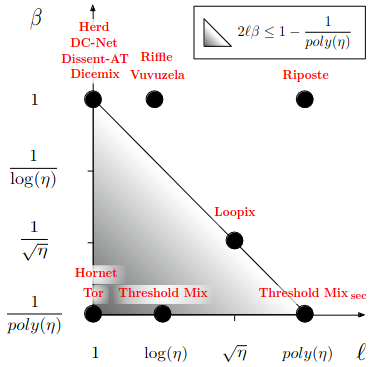
\includegraphics[scale=1.2]{triangle.png}
    %\caption{Caption}
    %\label{fig:enter-label}
\end{figure}



\vfill



\pagebreak


\subsection{Privacy Notions}

In the \textit{Mixnets basics} section, we provided an intuitive introduction to terms like \textit{unlinkability} and \textit{unobservability}. We can define these terms formally. In published literature, these are typically referred to as \textit{privacy notions}. Several papers endeavored to provide a formal framework for these notions. \citeE{analysis1} classified them in a hierarchy, the gist of which is "unobservability implies unlinkability, both-sides unlinkability implies each sender unlinkability and receiver unlinkability etc." Not all of the claims of the hierarchy are correct, and in the paper they are artifacts of the way the proofs are constructed as adversary-challenger games with some arbitrary choices made along the way. But to be fair, all papers exploring this question fall into that trap. The shortcomings of this paper are explored in the Extended Commentary section at the end of this work, including questionable framework, incorrect phrasing and straight up math mistakes. 
\medskip

\noindent We will now propose a straightforward definition of anonymity notions in terms of probability from the point of view of the observer. This is a direct application of Kolmogorov relations, although in anonymity literature it is sometimes attributed to \citeE{anoa}, crediting them for re-inventing the wheel.\footnote{Admittedly, this problem goes both ways as some of the greatest minds in probability theory claimed to introduce the entire field of anonymity in 2014 \citeE{pete}, with a fresh but not very useful angle and a cute new name - \textit{cryptogenography}.
}\medskip


\noindent  In probability theory, randomness is always in the eye of the beholder and so observer-specific uncertainty is an essential way to define it without arbitrary and controversial restrictions. Defining an anonymity notion obeys the following pattern. Suppose that the adversary $\mathcal{A}$ makes a guess whether an event $X$ occurred based on the available information. 

$\mathbb{P}[X_\mathcal{A}]$ is the probability that $X$ occurred based on the information available to $\mathcal{A}$. 

$\mathbb{P}[X_\mathcal{A}|X]$ is the probability that $X$ occurred according to $\mathcal{A}$, provided that $X$ actually occurred, 

$\mathbb{P}[X_\mathcal{A}|X']$ as the probability that $X$ occurred according to $\mathcal{A}$, provided that $X$ did not occur. 

\noindent We would like to say that for some $\delta\geq 0$ small enough to satisfy our anonymity requirements, $$|\mathbb{P}[X_\mathcal{A}|X]-\mathbb{P}[X_\mathcal{A}|X']|\leq \delta.$$ In a perfect system, we would like $\delta=0$, which would mean that the adversary $\mathcal{A}$ has exactly the same knowledge whether the event $X$ occurred or not with probability 1, which would make the event $X$ and the event of the adversary guessing that $X$ occurred independent events. \medskip

\noindent If $\mathbb{P}[X_\mathcal{A}|X]>\mathbb{P}[X_\mathcal{A}|X']$, we refer to the difference as the \textit{adversary advantage.}\medskip

\noindent The event $X$ could then be:
\begin{itemize}
    \item $X:=$ message $m$ exists. For message unobservability.
    \item $X:=$ User $A$ communicates with User $B$. For sender-receiver unlinkability.
    \item $X:=$ User $A$ sent the message $m.$ For sender-message unlinkability.
    \item $X:=$ User $A$ sent a message. For sender unobservability.
    \item $X:=$ User $B$ received the message $m.$ For receiver-message unlinkability.
    \item $X:=$ User $B$ received a message. For receiver unobservability.
\end{itemize}\medskip

\noindent In the Extended Commentary section, we go through an example in detail, by calculating adversary advantage on the receiver observability in Loopix. 

\pagebreak

\newpage
\section{Extended commentary on the published research (by E. J. Infeld)}
%This section might as well be called "Eva has no patience for people misusing mathematics." I take full responsibility for the criticism that follows. - EJI

\subsection{Loopix}
\subsubsection{(Failed) memorylessness of the mix}
As promised in our summary of the Loopix design, we will now explore the relationship between the exponential distribution and Poisson processes, in order to convince the reader the name \textit{Poisson mix} should be changed to \textit{Memoryless mix\textbf{ing}} instead. And like much in probability theory, it all starts with a coin toss.\medskip

\noindent Suppose we are tossing a coin, and it lands on heads with $1/2$ probability and tails with the remaining $1/2$ probability. And suppose we will keep tossing it until the first time it lands on heads, and then stop. Let the total number of tosses, finishing with the first toss that lands heads, be the discrete random variable $X$. An astute student of probability will know, that the probability of the first toss landing heads is $1/2$, the first landing tails and then second landing heads is $1/4$, and so on, with the probability of the the first $i-1$ tosses landing tails and and $i$th landing heads being $(1/2)^i$. So the probability distribution of how many tosses it will take for us to stop tossing the coin decays exponentially. Suppose we are making these tosses at a rate of one toss per second.

\begin{figure}[ht!]
    \centering
    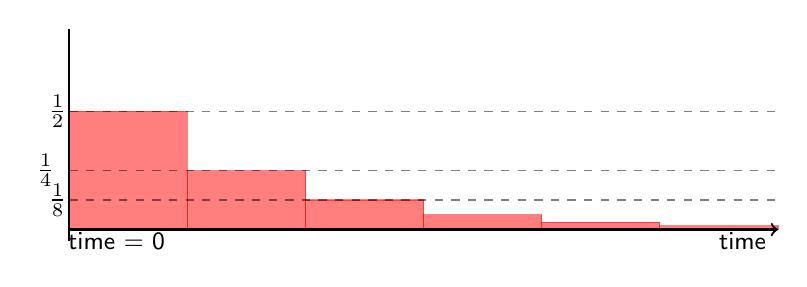
\begin{tikzpicture}[scale=3]

\foreach \x in {1,2,3,4,5,6}{
\filldraw[red,opacity=0.5] (\x*0.5-0.5,0) rectangle (\x*0.5,0.5^\x);}
\draw (-0.05,0.5) node {$\frac{1}{2}$};
\draw (-0.1,0.25) node {$\frac{1}{4}$};
\draw (-0.05,0.125) node {$\frac{1}{8}$};
\draw[dashed, opacity=0.5] (0,0.5) -- (3,0.5);
\draw[dashed, opacity=0.5] (0,0.25) -- (3,0.25);
\draw[dashed, opacity=0.5] (0,0.125) -- (3,0.125);
\foreach \t in {3}{
\draw[thick,->] (0,0) -- (\t,0);
\draw[thick] (0,0.85) -- (0,-0.05);
\draw (0.2,-0.05) node {\small time = 0};
\draw (\t-0.15,-0.05) node {\small time};}
    \end{tikzpicture}
    %\caption{Caption}
    %\label{fig:enter-label}
\end{figure}

\noindent The expected number of tosses we make is then: $$\mathbb{E}[X]=\sum_{i=1}^{\infty}\frac{1}{2^i}\times i=\sum_{i=1}^{\infty}\frac{1}{2^i}+\sum_{i=2}^{\infty}\frac{1}{2^i}+\sum_{i=3}^{\infty}\frac{1}{2^i}+\dots=$$ $$=1\times\sum_{i=1}^{\infty}\frac{1}{2^i}+\frac{1}{2}\times\sum_{i=1}^{\infty}\frac{1}{2^i}+\frac{1}{4}\times\sum_{i=1}^{\infty}\frac{1}{2^i}  =$$ $$=\left(1+\frac{1}{2}+\frac{1}{4}+\dots\right)\sum_{i=1}^{\infty}\frac{1}{2^i}=2\times 1 =2.$$

\noindent We can refer to this process formally as consecutive Bernoulli trials until first success. Now suppose that instead we are making coin tosses at the rate of every half a second, but the probability of the coin landing heads is $1/4$. The expected number of tosses, calculated the same way, is $4$, but since our time increment is now half a second, the expected time to success is still $2$ seconds.


%\begin{figure}[ht!]
%    \centering
%    \begin{tikzpicture}[scale=4]

%\foreach \x in {0,1,2,3,4,5,6,7}{
%\filldraw[red,opacity=0.5] (\x*0.25,0) rectangle (\x*0.25+0.25,0.25*0.75^\x);}
%\draw (-0.15,0.187) node {$\frac{3}{16}$};
%\draw (-0.05,0.25) node {$\frac{1}{4}$};
%\draw[dashed, opacity=0.5] (-0.25,0.187) -- (2,0.187);
%\draw[dashed, opacity=0.5] (0,0.25) -- (2,0.25);
%\foreach \t in {2}{
%\draw[thick,->] (0,0) -- (\t,0);
%\draw[thick] (0,0.45) -- (0,-0.05);
%\draw (0.15,-0.05) node {\tiny time = 0};
%\draw (\t-0.15,-0.05) node {\tiny time};}
%    \end{tikzpicture}
    %\caption{Caption}
    %\label{fig:enter-label}
%\end{figure}

$$\mathbb{E}[X']=\sum_{i=1}^\infty \frac{1}{4}\times\left(\frac{3}{4}\right)^{i-1}\times i=\frac{1}{4}\times \sum_{i=0}^\infty \left(\frac{3}{4}\right)^{i}\times \sum_{i=0}^\infty \left(\frac{3}{4}\right)^{i}=\frac{1}{4}\times 4\times 4=4.$$

\noindent Both of these distributions decay geometrically, and the expected time to success is the same. We can continue this process - as the time increments get smaller and smaller and we decrease the probability of a successful toss accordingly to keep the expected time to success the same - these discrete distributions will tend to a continuous limit. That continuous limit is the exponential distribution $f(x)=\lambda e^{-\lambda x}$ with parameter $\lambda=\frac{1}{\mathbb{E}[X]}$.

\begin{figure}[!ht]
\centering\hfill
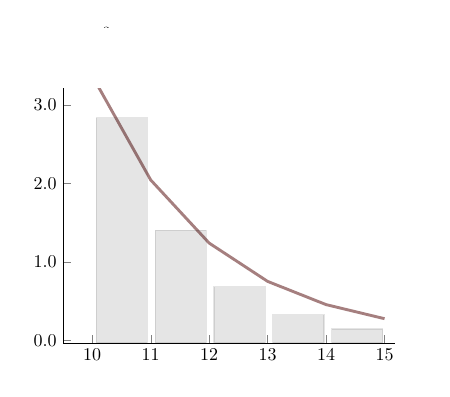
\begin{tikzpicture}[scale=0.65,declare function={exdec(\x,\l)=\l*exp(-\l*\x);}]
\begin{axis}[
    samples at={10,...,15},
    yticklabel style={
        /pgf/number format/fixed,
        /pgf/number format/fixed zerofill,
        /pgf/number format/precision=1
    }
]
\addplot [red!30!black, ultra thick,opacity=0.5] {exdec(x,0.5)};
\end{axis}
\filldraw[white] (6.5,6.15) rectangle (7,-0.5);
\filldraw[white] (7,6.15) rectangle (0,5);
\foreach \f in {0.88}{
\filldraw[opacity=0.1] (0.65,0) rectangle (1.65,5*\f);
\filldraw[opacity=0.1] (1.8,0) rectangle (2.8,2.5*\f);
\filldraw[opacity=0.1] (2.95,0) rectangle (3.95,1.25*\f);
\filldraw[opacity=0.1] (4.1,0) rectangle (5.1,0.63*\f);
\filldraw[opacity=0.1] (5.25,0) rectangle (6.25,0.31*\f);
}
\end{tikzpicture}
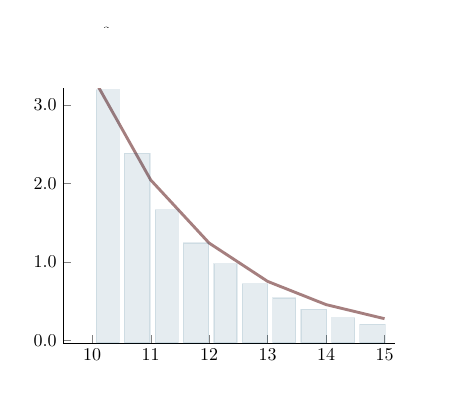
\begin{tikzpicture}[scale=0.65,declare function={exdec(\x,\l)=\l*exp(-\l*\x);}]
\begin{axis}[
    samples at={10,...,15},
    yticklabel style={
        /pgf/number format/fixed,
        /pgf/number format/fixed zerofill,
        /pgf/number format/precision=1
    }
]
\addplot [red!30!black, ultra thick,opacity=0.5] {exdec(x,0.5)};
\end{axis}
\filldraw[white] (6.5,6.15) rectangle (7,-0.5);
\filldraw[white] (7,6.15) rectangle (0,5);
\foreach \f in {0.88}{

\filldraw[opacity=0.1, blue!50!black] (0.65,0) rectangle (1.1,5.625*\f);
\filldraw[opacity=0.1, blue!50!black] (1.2,0) rectangle (1.7,4.21*\f);
\filldraw[opacity=0.1, blue!50!black] (1.8,0) rectangle (2.25,2.96*\f);
\filldraw[opacity=0.1, blue!50!black] (2.35,0) rectangle (2.85,2.22*\f);
\filldraw[opacity=0.1, blue!50!black] (2.95,0) rectangle (3.4,1.76*\f);
\filldraw[opacity=0.1, blue!50!black] (3.5,0) rectangle (4,1.32*\f);
\filldraw[opacity=0.1, blue!50!black] (4.1,0) rectangle (4.55,1*\f);
\filldraw[opacity=0.1, blue!50!black] (4.65,0) rectangle (5.15,0.75*\f);
\filldraw[opacity=0.1, blue!50!black] (5.25,0) rectangle (5.7,0.56*\f);
\filldraw[opacity=0.1, blue!50!black] (5.8,0) rectangle (6.3,0.42*\f);
}
\end{tikzpicture}
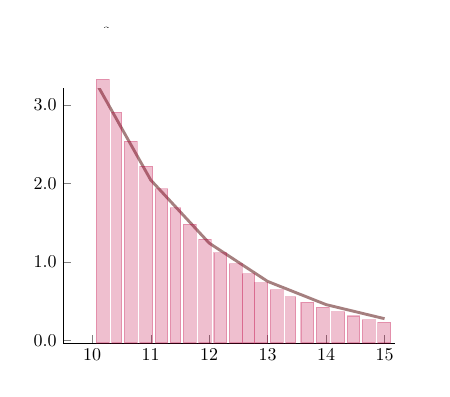
\begin{tikzpicture}[scale=0.65,declare function={exdec(\x,\l)=\l*exp(-\l*\x);}]
\begin{axis}[
    samples at={10,...,15},
    yticklabel style={
        /pgf/number format/fixed,
        /pgf/number format/fixed zerofill,
        /pgf/number format/precision=1
    }
]
\addplot [red!30!black, ultra thick,opacity=0.5] {exdec(x,0.5)};
\end{axis}
\filldraw[white] (6.5,6.15) rectangle (7,-0.5);
\filldraw[white] (7,6.15) rectangle (0,5);
\foreach \f in {0.88}{
%\filldraw[white] (0,0.15) rectangle (7,-0.5);
\filldraw[opacity=0.25, purple] (0.65,0) rectangle (0.9,5.86*\f);
\filldraw[opacity=0.25, purple] (0.95,0) rectangle (1.15,5.125*\f);
\filldraw[opacity=0.25, purple] (1.2,0) rectangle (1.45,4.48*\f);
\filldraw[opacity=0.25, purple] (1.5,0) rectangle (1.75,3.92*\f);
\filldraw[opacity=0.25, purple] (1.8,0) rectangle (2.05,3.43*\f);
\filldraw[opacity=0.25, purple] (2.1,0) rectangle (2.3,3*\f);
\filldraw[opacity=0.25, purple] (2.35,0) rectangle (2.6,2.637*\f);
\filldraw[opacity=0.25, purple] (2.65,0) rectangle (2.9,2.3*\f);
\filldraw[opacity=0.25, purple] (2.95,0) rectangle (3.2,2*\f);
\filldraw[opacity=0.25, purple] (3.25,0) rectangle (3.5,1.76*\f);
\filldraw[opacity=0.25, purple] (3.5,0) rectangle (3.75,1.54*\f);
\filldraw[opacity=0.25, purple] (3.75,0) rectangle (4,1.34*\f);
\filldraw[opacity=0.25, purple] (4.05,0) rectangle (4.3,1.18*\f);
\filldraw[opacity=0.25, purple] (4.35,0) rectangle (4.55,1.03*\f);
\filldraw[opacity=0.25, purple] (4.65,0) rectangle (4.9,0.9*\f);
\filldraw[opacity=0.25, purple] (4.95,0) rectangle (5.2,0.79*\f);
\filldraw[opacity=0.25, purple] (5.25,0) rectangle (5.5,0.69*\f);
\filldraw[opacity=0.25, purple] (5.55,0) rectangle (5.8,0.6*\f);
\filldraw[opacity=0.25, purple] (5.85,0) rectangle (6.1,0.52*\f);
\filldraw[opacity=0.25, purple] (6.15,0) rectangle (6.4,0.46*\f);
}
\end{tikzpicture}\hfill\hfill
\caption{Probability distributions of first success in consecutive Bernoulli trials, starting at $t=10s$ (because the first terms are messy and don't matter in the limit) for probability of success 0.5, 0.25 and 0.125 respectively, with time increments decreased accordingly, plotted against the exponential distribution with $\lambda=0.5$.}
\end{figure}

\noindent The process of repeatedly tossing a coin until it comes up heads is memoryless - it doesn't matter how many times you already got tails, if you're still tossing, the probabilities for the next toss are the same. Similarly, if a mix node was repeatedly rolling dice to release a message in the next (very small) time increment with probability $p$, how long the message will be waiting till release would not depend on how long it has already been sitting there. If we imagine that at time $t'$ there are $k$ messages sitting at a mix node, and we're rolling dice independently for each to either release it or not, it would not matter in what order these messages arrived at the node, or how long ago. And so the first outgoing message could be any one of them with uniform probability. In its continuous approximation this is the mix that employs independent exponential delays.\medskip

\noindent Now, a Poisson process is a series of events of this type distributed in time. This again relates to the coin toss (or, more formally, Bernoulli trials.) If we were tossing the coin relentlessly, not stopping at any point, the event of the coin coming up heads could be marked on a time axis like so:

\begin{figure}[ht!]
    \centering
    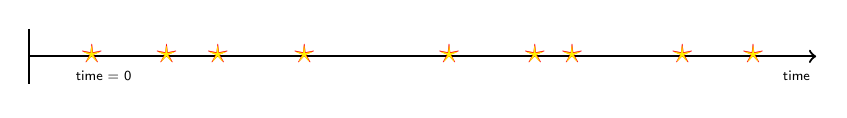
\begin{tikzpicture}
        \foreach \t in {10}{
\draw[thick,->] (0,0) -- (\t,0);
\draw[thick] (0,0.35) -- (0,-0.35);
\draw (0.95,-0.25) node {\tiny time = 0};
\draw (\t-0.25,-0.25) node {\tiny time};}
\foreach \x in {0.8,1.75,2.4,3.5,5.34, 6.427,6.9,8.3,9.2}{\draw[red] (\x,0.025) node {\Large $\star$}; \draw[yellow] (\x,0.025) node {\large $\star$};}
    \end{tikzpicture}
    %\label{fig:enter-label}
\end{figure}

\noindent The limit of the process of tossing the coin with a set expected time to success at smaller and smaller time increments and decreasing the probability $p$ proportionally, is called a Poisson process. There are countless things in nature that can be modelled this way, for example particle decay. The distances between consecutive events are sampled from the exponential distribution. On the other hand, a Poisson distribution describes how many events of this nature occurred in a time for which the expected number of events is some parameter $\lambda$. Since it's counting, the Poisson distribution itself is not memoryless.

Poisson processes are common, and likewise there are many ways to set up a relay releasing messages to look like a Poisson process. It could first roll the dice on whether to release a message or not, and then on success choose which message according to any algorithm. It could even be a queue, in which case we don't achieve any mixing. Or it could choose the message uniformly at random, in which case we do.

On the other hand, in the Loopix model, each message has its own independent exponential delay. The overall behavior of a mix node isn't necessarily a Poisson process, because depending on the number of messages in the system, and the node itself, the expected delay to the next message being released from a node is likely to fluctuate. The overall behavior will only be Poisson distributed if the number of messages in a node at each point can be approximated to be constant. So not only does the name \textit{Poisson mix} not correspond to the memorylessness of the setup, it's not even true. That's why we insist on calling it \textit{memoryless mixing} instead.


\subsubsection{Receiver observability (by compromised provider or provider-receiver traffic)}

The direct receiver observability in Loopix has been openly discussed and somewhat downplayed by the authors. If Bob is receiving messages, and Bob's provider is compromised, then whenever Bob is offline the provider can tell with full certainty that Bob received a message. While Bob is online, there are also Bob's loop decoys coming back which may look the same to the provider, however, they have their own independent distribution and so the legitimate messages can be detected with simple statistical analysis, for example basic signal processing. The same process can be employed by and adversary who instead of compromising the provider, is watching the incoming connections to Bob, if no padding of the provider's response is employed.

Let us calculate the adversary advantage to drive the point home. Suppose that Bob is receiving his own loop decoys coming back at the average rate of $2$ in time $t$, and that the adversary guesses, before seeing the traffic, that the probability of Bob receiving a legitimate message in that time period is $0<p<1$.

Suppose that in the time window $t_0$ of length $t$ Bob received $k$ packets. An adversary will then adjust their perceived probability on whether one of these was likely to be a non-loop message. In this case, since the background process are just loop decoys generated by Bob, it is in fact Poisson distributed and so the adversary advantage is easy to calculate. The two distributions are now: $$\mathbb{P}_0[k]=e^{-2}\frac{2^k}{k!}\bigg|_{k\geq 0}\text{ if Bob did not receive a message, and }\mathbb{P}_1[k]=e^{-2}\frac{2^{k-1}}{k!}\bigg|_{k\geq 1}\text{ if he did.}$$ If Bob received zero packets, we can conclude he did not receive the message. However, if he received, say, 3 packets, that corresponds to a distribution term $2e^{-2}$ if he received a message, and $\frac{4}{3}e^{-2} $if he did not. If the adversary judges the probability of Bob receiving a message during the time $t_0$ before observing the traffic as $p,$ and since the two types of traffic are independent, we are left with the conditional probability: $$p'_3=\frac{p\times 2e^{-2}}{p\times 2e^{-2}+(1-p)\times\frac{4}{3}e^{-2}}=p\times \frac{1}{p+(1-p)\times \frac{2}{3}}=p\times\frac{3}{2+p}>p,$$ and so the adversary has an advantage over the previous guess. In fact, if we observe $k\geq 1$ packets coming in: $$p'_k=p\times \frac{k}{2+(k-2)\times p},$$ and the only term for which the adversary advantage is 0 turns out to be that for $k=2$, with $p'_2=p$. The number 2 was chosen arbitrarily, we could choose any positive real number and adjust $p$ and $t$ accordingly.

%We can even calculate the expected adversary advantage: $$(1-p)e^{-2}+\sum_{k\geq 1}|p'_k-p|\left(p\frac{2^{k-1}e^{-2}}{(k-1)!}+(1-p)\frac{2^{k}e^{-2}}{(k)!}\right)$$

How significant that advantage is in absolute terms will depend on $p$, in other words, it will depend on the ratio of legitimate message traffic to loop decoy traffic. If there is any regularity to the legitimate message traffic, however, the adversary will detect it, over time, with probability approaching 1.

Modern implementations have introduced mitigation tactics, such as padding the response every time a user queries their provider. In this case, there are still concerns about the fact that this protection is entirely lost if the provider is compromised, and from the fact that the act of querying the provider remains observable, and Bob's pattern of querying is likely to leak whether a message was received or not. 

\pagebreak
\subsubsection{Independent legitimate traffic bug}

There is another very serious issue that doesn't seem to be getting any attention. A legitimate message or returning loop going from the last layer of mixes is sure to go to the receiver's provider, as opposed to all other traffic from the last layer of mixes, which is uniformly distributed among providers. This means that legitimate traffic at that hop is also observable, as long as it is statistically significant. In particular, if there is a regularity to it, it will be detectable with probability 1. This is very dangerous even in short term, since the low latency between the sender and the receiver's provider opens this system to correlation attacks, and any advantage that comes from messages being asynchronous is lost.

\begin{figure}[!ht]
\centering
\begin{tikzpicture}[scale=2.25]
\foreach \N in {0,1.5,3}{
\draw [->,blue!50!gray,opacity=1] plot [smooth, tension=1] coordinates { (-0.75-\N*0.1,1.2) (0+\N*0.2,2.5+\N*0.2) (\N+0.5,2.5)};
\foreach \L in {0,1,2}{
\draw [->,blue!50!gray,opacity=0.35] plot [smooth, tension=1] coordinates { (\N+0.5+\L*0.1,0) (-\N*0.1-0.2*\L,-\N*0.2+\L*0.5) (-0.8-\N*0.1,\L+0.1)};}
}
\draw[blue!25!black] (-3,1.65) node {Alice};
\draw[blue!25!black] (-1,0.85) node {Alice's provider};
\draw[blue!25!black] (-1,-0.15) node {Bob's provider};
\node[client, minimum size=1cm] at (-3,0.5) {};
\node[client, minimum size=1cm] at (-3,2) {};
\draw[blue!25!black] (-3,0.2) node {Bob};
\foreach \L in {-0,1,2}{
\node[server, fill=purple!50!blue, minimum size=1.5cm] at (-1,\L+0.25) {};
%\draw[blue!25!black] (5,2-\L+0.25) node {$L_{\L}$};
\foreach \N in {0,1.5,3}{
\node[server, fill=blue!50!black, minimum size=1.5cm] at (\N+0.5,\L+0.25) {};
%\draw[rounded corners,blue!25!black] (\N,\L) rectangle (\N+1,\L+0.5);
}}
\foreach \L in {0,1}{
%\draw (5,\L+0.75) node {$\vdots$};
\foreach \N in {0,1.5,3}{
\foreach \k in {0,1.5,3}{
\draw[->, blue!50!gray, opacity=0.35] (\N+0.5,\L+1) -- (\k+0.5,\L+0.6);
}}}
\draw [->,black!50!blue,ultra thick] plot [smooth, tension=1] coordinates { (-2.75,2) (-1.3,1.25)};
\draw [->,black!50!blue,thick,opacity=0.5] plot [smooth, tension=1] coordinates { (-1.3,0.25) (-2.75,0.45)};
\draw [->,blue!50!black,opacity=1] plot [smooth, tension=1] coordinates { (3+0.5+0.1,0) (-3*0.1,-3*0.2) (-0.8-3*0.1,0.1)};
\end{tikzpicture}
\caption{The distribution of Alice's traffic, as she communicates with Bob. The providers are marked in purple, and mix nodes in blue. The increase in traffic to Bob's provider when Bob receives a message is observable.}
\end{figure}

A simple way of addressing this problem if there aren't too many providers is for the client who wants to send a message to a specific provider to wait for a decoy packet that would naturally be going to the same provider and instead send the message. This increases the overall expected first-hop latency by a factor of $P$, adding $(P-1)\times\frac{1}{\lambda}$ to the over all expected latency, where $P$ is the number of providers and $\lambda$ is the parameter chosen for the message delay. Another way of looking at the trade-off is that the effective bandwidth to every provider is reduced by a factor of $P$, which is particularly bothersome if we are trying to send a large file consisting of multiple packets. However, that is exactly when this bug is the most dangerous - sending a large file will always be observable.

This fix couples the decoy and message traffic in a fully unobservable way, and so despite its trade-offs it should be implemented it to save the anonymity in the system.

%\subsection{Anonymity Trilemma}
%\citeE{trilemma} claims to prove the relation and provide the following upper bound on an anonymity factor $\eta$: $$2\beta \ell\geq 1-\frac{1}{P(\eta)},$$ where $\beta$ is the bandwidth overhead, $\ell$ is latency and $P(\eta)$ is polynomial in $\eta.$\medskip

%\noindent Right away we notice that the bound is asymptotic, and yet the factor of 2 is left in, which doesn't bode well for the tightness of the paper.
\vfill

\pagebreak
\subsection{Privacy Notions}

I feel compelled to point out a few shortcomings of \citeE{analysis1}. The paper is very hand-wavy, which is unacceptable for a work that claims to provide a formal framework. Let's consider a paragraph already on page 3:\bigskip

\parbox{45em}{(...) Thus, we need to show for the applied protection measure, that compared to any other sender of the message, it is not more probable that Alice is the sender. We analyze the worst case: in a group of users, let Charlie be a user for whom the probability of being the sender differs most from Alice's probability. If even these are too close to distinguish, Alice is safe, since all other probabilities are closer.} 

\bigskip

This paragraph should never have made it into a research publication. One, it should say "any other \textit{possible} sender of the message." Two, it starts out saying "it is not more probable" to then assume it is in fact the most probable, but all other probabilities are withing an error margin, which it doesn't say explicitly. A reader would not be wrong to wonder, what if Charlie's perceived probability is, in fact, higher, which it fails to either account for or exclude, but which can very much happen in practice. It also fails to adequately define what "probable" means, even though the paper does mention an adversary observer much earlier, so we are meant to fill in the gaps. 

Unfortunately, the rest of the paper isn't much better.On pages 5 and 6, we have a math error with "0" an "1" transposed. There is a claim that $$\left| Pr[0=\langle\mathcal{A}|Ch(\Pi,X,c,0) \rangle]-Pr[0=\langle\mathcal{A}|Ch(\Pi,X,c,1) \rangle]\right|\leq\delta$$ is equivalent to the following two equations together: $$ Pr[0=\langle\mathcal{A}|Ch(\Pi,X,c,0) \rangle]\leq Pr[0=\langle\mathcal{A}|Ch(\Pi,X,c,1) \rangle]+\delta,$$
$$ Pr[1=\langle\mathcal{A}|Ch(\Pi,X,c,1) \rangle]\leq Pr[1=\langle\mathcal{A}|Ch(\Pi,X,c,0) \rangle]+\delta.$$ But these two latter equations mean the same thing. The authors appear to have meant the last one to be:  $$ Pr[1=\langle\mathcal{A}|Ch(\Pi,X,c,0) \rangle]\leq Pr[1=\langle\mathcal{A}|Ch(\Pi,X,c,1) \rangle]+\delta.$$ This is a trivial argument that is stretched to an entire section, one might as well try to get it right. \medskip

\noindent The paper's nomenclature is messy, inconsistent, and needlessly complicated, and uses words and symbols customarily used differently in mathematics. It defines some of the notions with arbitrary restrictions, say, from page 8 on it is clear that its definition of sender-receiver linkability requires that the adversary identifies a specific message from the sender to the receiver, which should not be a requirement, least of all in a probabilistic setting. You don't need to identify a specific message to know that they exist.

This is an artifact of the framework, and only one of the issues with it. Defining anonymity in terms of adversary-specific indistinguishability is natural, and has been widely explored in probabilistic combinatorics. But the game constructs in the paper are contrived and arbitrary. This ripples through the paper, and affects the resulting hierarchy. There are relations in it that are blatantly false, such as, to stick to the above example, a claim that sender-receiver linkability implies message observability, which the reader hopefully accepts is nonsense.

And even more outrageous problem is that the relation described in the hierarchy is incorrectly described as an implication, rather than a marking stricly stronger property, leading us to follow through the graph to conclusions like "message unobservability implies message observability," which is clearly false.



\section{Bibliography}

\bibliographystyleM{unsrt}
\bibliographyM{research}

\bibliographystyleA{unsrt}
\bibliographyA{attacks}

\bibliographystyleE{unsrt}
\bibliographyE{evaluation}






\end{document}

Between the last layer and the receipient's provider you can observe and increase in packets going to that provider

\begin{figure}[!ht]
\begin{tikzpicture}
\foreach \x in {(0,-3),(0.5,-2),(0,-1),(-1,-2.75),(-0.35,-2),(-0.75,-0.5),(0.8,-0.85),(-0.8,0.3)}{
\draw[dashed] \x circle (10pt);}
\draw (0.5,0) node {Alice};
\draw[dashed] (0.5,0) circle (15pt);
\draw (0.2,1.2) node {Bob};
\draw[dashed] (0.2,1.2) circle (15pt);

\foreach \x in {(7.5,-0.75), (9,0.5)}{
\draw[opacity=0.5] \x circle (15pt);
}


\draw[thick,->] (1.3,0)--(7.7,-3.2);

\filldraw[white] (3.75,-2.4) rectangle (6.25,-0.25);
\draw[rounded corners] (4.2,-2) rectangle (5.8,-1.3);
\draw (5,-1.6) node {Hello!};
\draw[rounded corners, opacity=0.75] (4,-2.2) rectangle (6,-0.8);
\draw (5,-1) node {send to Bob};
\draw[rounded corners, opacity=0.5] (3.75,-2.4) rectangle (6.25,-0.25);
\draw (5,-0.5) node {send to 4};
%\draw[rounded corners, opacity=0.25] (3.5,-2.5) rectangle (6.5,0.25);
%\draw (5,0) node {send to 25};

\filldraw[white] (8.3,-3.5) circle (15pt);
\draw (8.3,-3.5) circle (15pt);
\draw (8.3,-3.5) node {25};

\draw[thick,->] (8.9,-3.2) -- (11.9,-0.2);

\filldraw[white] (9,-2.2) rectangle (11,-0.8);
\draw[rounded corners] (9.2,-2) rectangle (10.8,-1.3);
\draw (10,-1.6) node {Hello!};
\draw[rounded corners, opacity=0.75] (9,-2.2) rectangle (11,-0.8);
\draw (10,-1) node {send to Bob};

\filldraw[white] (12.4,0.3) circle (15pt);
\draw (12.4,0.3) circle (15pt);
\draw (12.4,0.3) node {4};

\draw[thick,->] (11.7,0.3) -- (0.85,1.2);
\filldraw[white] (6,-) rectangle (8,0.95);
\draw[rounded corners] (6.2,0.2) rectangle (7.8,0.9);
\draw (7,0.6) node {Hello!};
\end{tikzpicture}
\end{figure}



\end{figure}


\begin{figure}[!ht]
\centering
\begin{tikzpicture}[scale=0.7]

\foreach \x in {(0,-2),(0.85,-1),(-1.25,-1.75),(-0.35,-1),(-0.75,0.5),(0.8,1.25),(-0.8,2.2)}{
\node[client, minimum size=0.7cm] at \x {};
}

\draw [->,black!25!blue,ultra thick] plot [smooth, tension=1] coordinates { (0.75,-2.25) (3.5,-3.2) (4.5,-3) (6.5,-1.5)};
\draw [->,black!25!cyan,ultra thick] plot [smooth, tension=1] coordinates { (1.4,1)  (3.75,-1.5) (5.9,-1.2)};
\draw [->,black!25!cyan,ultra thick] plot [smooth, tension=1] coordinates { (6.3,0) (3.1,0.8) (1,2.3) (-0.2,2.1)};
\draw [->,black!50!blue,ultra thick] plot [smooth, tension=1] coordinates { (6.5,0.35)  (3.6,2.2) (0.5,2) (-0.4,1)};


\draw (0.75,0.5) node {Alice};
\draw (-0.95,1.45) node {Bob};
\draw (0,-2.75) node {Charlie};
\draw (-0.75,-0.1) node {Diane};

\foreach \x in {(3.1,0.8)}{
\node[messageclosed, fill=cyan!15, draw=black!40,minimum size=1.2cm] at \x {};}

\foreach \x in {(3.6,2.2)}{
\node[messageclosed, fill=blue!10!purple!10, draw=black!40,minimum size=1.2cm] at \x {};}

\foreach \x in {(3.5,-2.9),(3.75,-0.9)}{
\node[messageclosed, fill=green!15, draw=black!40,minimum size=1.75cm] at \x {};}

\draw (3.6,2.2) node {Hello!};
\draw (3.1,0.8) node {Hi :)};
\draw (3.5,-3.2) node {Hello!};
\draw (3.5,-2.5) node {send to 11};
\draw (3.75,-1.2) node {Hi :)};
\draw (3.75,-0.4) node {send to 01};


\node[server, minimum size=2cm, fill=green!50!gray] at (7.5,-0.5) {};
\filldraw[red, opacity=0.2] (6.5,2.8) rectangle (9.5,2.1);
\filldraw[blue, opacity=0.2] (6.5,1.5) rectangle (9.5,2.1);
\filldraw[magenta, opacity=0.2] (6.5,1.5) rectangle (9.5,1);
\filldraw[purple!50!blue, opacity=0.2] (6.5,0.5) rectangle (9.5,1);
\draw[gray!50] (6.5,2.8) rectangle (9.5,0.5);
\draw (8,2.35) node {Alice=00};
\draw (8,1.85) node {Bob=01};
\draw (8,1.35) node {Charlie=10};
\draw (8,0.85) node {Diane=11};


\end{tikzpicture}
\hfill
\begin{tikzpicture}[scale=0.7]

\foreach \x in {(0,-2),(0.85,-1),(-1.25,-1.75),(-0.35,-1),(-0.75,0.5),(0.8,1.25),(-0.8,2.2)}{
\node[client, minimum size=0.7cm] at \x {};
}

\draw [->,black!25!blue,ultra thick] plot [smooth, tension=1] coordinates { (0.75,-2.25) (3.5,-3.2) (4.5,-3) (6.5,-1.5)};
\draw [->,black!25!cyan,ultra thick] plot [smooth, tension=1] coordinates { (1.4,1)  (3.75,-1.5) (5.9,-1.2)};
\draw [->,black!25!cyan,ultra thick] plot [smooth, tension=1] coordinates { (6.3,0) (3.1,0.8) (1,2.3) (-0.2,2.1)};
\draw [->,black!50!blue,ultra thick] plot [smooth, tension=1] coordinates { (6.5,0.35)  (3.6,2.2) (0.5,2) (-0.4,1)};

\node[messageclosed, minimum size=2cm, fill=green!15, draw=black!30] at (3.5,-3.1) {};
\node[messageclosed, minimum size=2cm, fill=green!15, draw=black!30] at (3.75,-1) {};


\draw (0.75,0.5) node {Alice};
\draw (-0.95,1.45) node {Bob};
\draw (0,-2.75) node {Charlie};
\draw (-0.75,-0.1) node {Diane};

\foreach \x in {(3.1,0.8),(3.75,-1.2)}{
\node[messageclosed, fill=cyan!15, draw=black!40,minimum size=1.2cm] at \x {};}

\foreach \x in {(3.5,-3.3),(3.6,2.2)}{
\node[messageclosed, fill=blue!10!purple!10, draw=black!40,minimum size=1.2cm] at \x {};}

\draw (3.6,2.2) node {Hello!};
\draw (3.1,0.8) node {Hi :)};
\draw (3.5,-3.2) node {Hello!};
\draw (3.5,-2.5) node {send to 11};
\draw (3.75,-1.2) node {Hi :)};
\draw (3.75,-0.4) node {send to 01};


\node[server, minimum size=2cm, fill=green!50!gray] at (7.5,-0.5) {};
\filldraw[red, opacity=0.2] (6.5,2.8) rectangle (9.5,2.1);
\filldraw[blue, opacity=0.2] (6.5,1.5) rectangle (9.5,2.1);
\filldraw[magenta, opacity=0.2] (6.5,1.5) rectangle (9.5,1);
\filldraw[purple!50!blue, opacity=0.2] (6.5,0.5) rectangle (9.5,1);
\draw[gray!50] (6.5,2.8) rectangle (9.5,0.5);
\draw (8,2.35) node {Alice=00};
\draw (8,1.85) node {Bob=01};
\draw (8,1.35) node {Charlie=10};
\draw (8,0.85) node {Diane=11};


\end{tikzpicture}


